\tocchapter{Softwarearen garapenerako prozesu bateratua}

\section{Eskakizunen bilketa}
Gure aplikazioak eduki behar dituen eskakizun funtzionalak zehazteko, hau da, aktoreen beharrak zerrendatzeko, balio du eskakizunen bilketak. Gure kasuan aktore bakarra izango dugu, \textbf{erabiltzailea} hain zuzen ere. Hauek dira bere eskakizunak:
\subsection{Azpitituluen inguruko eskakizunak}
\begin{itemize}
\item ASS, SRT edo SUB motako azpitituluak irekitzea eta gordetzea.
\item Azpititulu fitxategi berriak sortzeko aukera.
\item TXT fitxategietatik dialogoak inportatzea.
\item Fitxategiaren goiburukoen edizioa.
\item Lerro bakoitzaren eremuen gaineko edizioa: aktorea, estiloa, testua, denborak, etab. aldatzea.
\item Lerroen gaineko eragiketak: gehitu, kendu, \textit{shift}, \textit{split}, \textit{join}, bikoiztu, etab.
\item Sintaxia nabarmendua erosoago lan egiteko: ASS komandoen identifikazioa eta koloreztatzea.
\end{itemize}
\subsection{\textit{Typesetting}-aren inguruko eskakizunak}
\begin{itemize}
\item Estilo editorea estilo berriak sortzeko edo daudenak aldatzeko.
\item Estilo kudeatzailea, estiloak gorde ahal izateko edo \textit{script} batean txertatzeko.
\end{itemize}
\subsection{Audio sinkronizazioren inguruko eskakizunak}
\begin{itemize}
\item Audio formatu desberdinak irekitzea (MP3 eta WAV gutxienez).
\item Audioaren uhin forma marraztea.
\item Uhin formaren gainean lerro bakoitzaren hasiera eta amaiera denborak aukeratzea.
\item Audioa erreproduzitzea honako modu hauetan:
	\begin{itemize}
	\item Osorik erreproduzitea.
	\item Lehenengo 500 milisegunduak erreproduzitzea.
	\item Azkenengo 500 milisegunduak erreproduzitzea.
	\item Aurreko 500 milisegunduak erreproduzitzea.
	\item Hurrengo 500 milisegunduak erroproduzitzea.
	\end{itemize}
\end{itemize}
\subsection{Tresna edo laguntzaileen inguruko eskakizunak}
\begin{itemize}
\item Karaokeen silabak sinkronizatzeko modua.
\item Karaokeen efektuak sortzeko tresna sinplea.
\item Itzulpenak egiteko laguntzailea.
\item Zuzentzaile ortografikoa.
\end{itemize}
\subsection{Bestelako eskakizunak}
\begin{itemize}
\item Lana periodikoki gordetzea modu automatikoan.
\item Dokumentu anitz irekita edukitzea aldi berean.
\item Undo/Redo aukerak.
\end{itemize}

\section{Analisia}
Nahiz eta programak zenbait formaturekin lan egin ahalko duen (ASS, SRT, SUB eta TXT), formatu \textit{natiboa} ASS izango da. Honen arrazoia zera da: ASS formatuak badauka SRT, SUB eta TXT formatuek eskaintzen duten guztia, baina alderantziz ez, hau da, ASS formatua askoz aurreratuagoa da. 

\begin{figure}[htp]
\begin{center}
%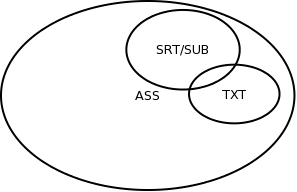
\includegraphics[width=\columnwidth, natwidth=555pt, natheight=402pt]{Pictures/Chapter4/Analisia/formatuak.png}
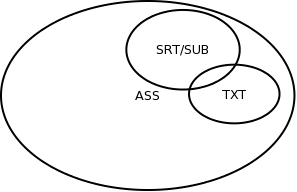
\includegraphics[scale=0.5]{Pictures/Chapter4/Analisia/formatuak.png}
\caption{Azpititulu formatuak}
\label{formatuak}
\end{center}
\end{figure}

\ref{formatuak}~Irudian ikusten denez, SRT, SUB eta TXT formatuak ASS formatuaren azpimultzoak direla esan daiteke. SUB eta SRT berdina eskaintzen dute, dialogoak eta hauen hasiera eta bukaera denborak. TXT formatuak ordea, dialogoak eta hauen aktoreak bakarrik eskaintzen ditu.
\subsection{Domeinuaren eredua}
\ref{de}~Irudian ikusten denez, domeinuko osagaien izenak ingeleraz daude, honako arrazoiengatik: alde batetik, ASS formatuaren espezifikazioan izenak ingeleraz agertzen direlako\cite{gu:ass}, eta bestetik programa askea izango denez, norbaitek kodea irakurri edo hobetu nahi badu, askoz errazagoa izango da ingelera jakitea euskera ordez.
\begin{figure}[htp]
\begin{center}
%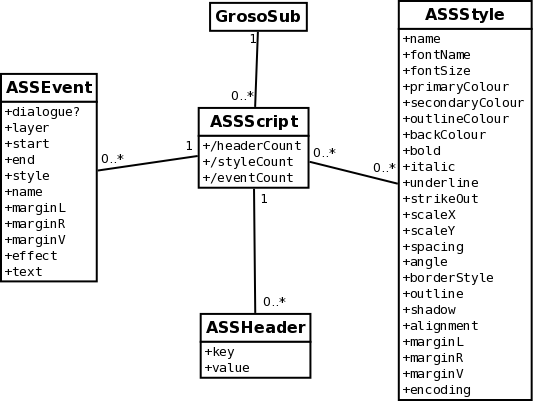
\includegraphics[width=\columnwidth, natwidth=555pt, natheight=402pt]{Pictures/Chapter4/Analisia/DE.png}
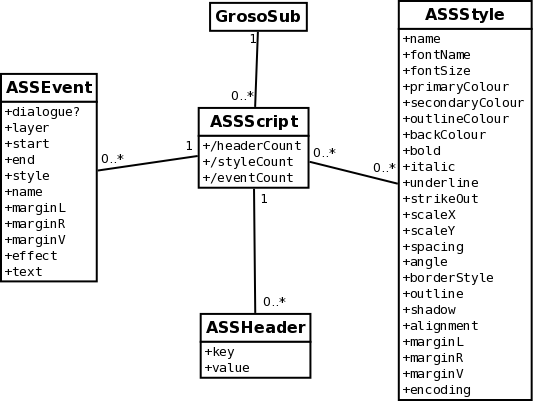
\includegraphics[scale=0.6]{Pictures/Chapter4/Analisia/DE.png}
\caption{Domeinuaren eredua}
\label{de}
\end{center}
\end{figure}

\subsection{Egoera diagrama}
Programaren izaera dela eta, egoera desberdinekin aurkituko gara. Definituko diren egoeratan zenbait erabilpen kasu gauzatu ahalko ditugu, batzutan beste egoera batzuetara pasaz. Honako diagrametan ikus daitezke egoerak eta hauen erabilpen kasuak:

\begin{figure}[htp]
\begin{center}
%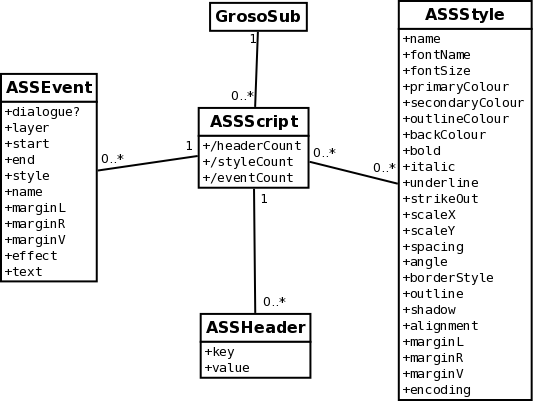
\includegraphics[width=\columnwidth, natwidth=555pt, natheight=402pt]{Pictures/Chapter4/Analisia/DE.png}
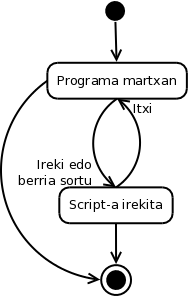
\includegraphics[scale=0.6]{Pictures/Chapter4/Analisia/ED.png}
\caption{Egoera diagrama}
\label{ed}
\end{center}
\end{figure}
\newpage
\subsection{Erabilpen kasuak}
\subsubsection{Egoera guztietan egin daitezkeenak}
\begin{figure}[htp]
\begin{center}
%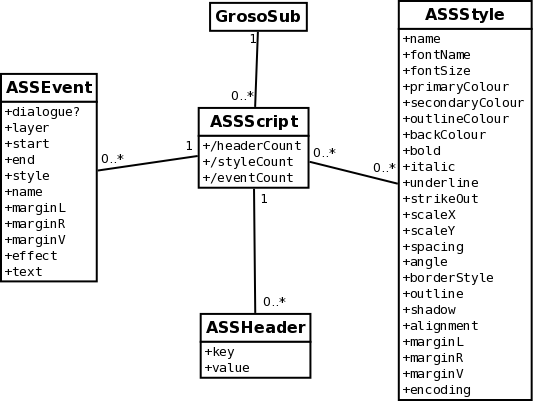
\includegraphics[width=\columnwidth, natwidth=555pt, natheight=402pt]{Pictures/Chapter4/Analisia/DE.png}
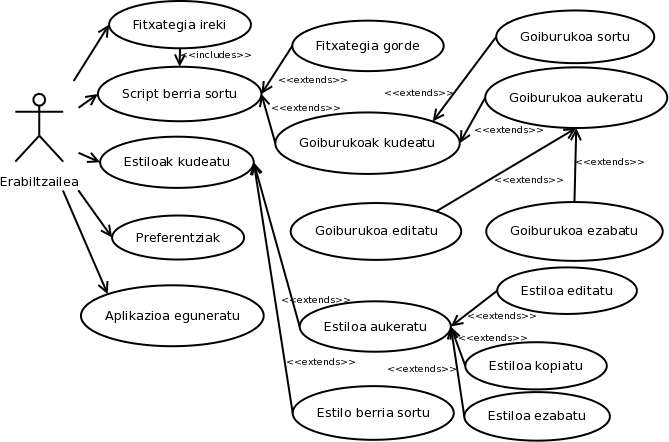
\includegraphics[scale=0.6]{Pictures/Chapter4/Analisia/EKE-Guztiak.png}
\caption{EKE - Egoera guztiak}
\label{eke-guztiak}
\end{center}
\end{figure}
\noindent\\
\textbf{ID:} G01.\\
\textbf{Erabilpen kasua:} Fitxategia ireki.\\
\textbf{Aktoreak:} Erabiltzailea.\\
\textbf{Deskribapena:} Fitxategi sisteman dagoen fitxategi bat kargatzen du.\\
\textbf{Aurrebaldintzak:} Fitxategia existitzen da.\\
\textbf{Postbaldintzak:} Fitxategia kargatuta geratzen da.\\
\textbf{Gertaera fluxu normala:}
\begin{enumerate}
	\item \textit{Erabiltzailea:} Fitxategi sistemako fitxategi bat aukeratzen du.
	\item \textit{Sistema:} Script berri bat sortzen du (\underline{includes: G02}).
	\item \textit{Sistema:} Sortu berri duen script-ean aukeratutako fitxategiko datuak kargatzen ditu.
	\item \textit{Sistema:} Erabiltzaileari erakusten dio lehio berri batean.
\end{enumerate}
\textbf{Gertaera fluxu alternatiboa:}
\begin{itemize}
	\item 3. urratsa: fitxategiaren formatua ez da zuzena.
		\begin{enumerate}
		\item \textit{Sistema:} Erabiltzaileari errorearen berri emango dio.
		\item \textit{Erabiltzailea:} Fitxategi berri bat aukeratuko du edo erabilpen kasutik aterako da.
		\end{enumerate}
\end{itemize}
\line(1,0){390}\\
\noindent\\
\textbf{ID:} G02.\\
\textbf{Erabilpen kasua:} Script berria sortu.\\
\textbf{Aktoreak:} Erabiltzailea.\\
\textbf{Deskribapena:} Script berri bat sortzen da defektuzko balioekin.\\
\textbf{Aurrebaldintzak:}\\
\textbf{Postbaldintzak:} Script-a sortzen da eta erabiltzaileari erakusten zaio.\\
\textbf{Gertaera fluxu normala:}
\begin{enumerate}
	\item \textit{Sistema:} Script berria sortzen du eta defektuzko informazioarekin osatzen du.
	\item \textit{Sistema:} Erabiltzaileari erakusten dio lehio berri batean.
\end{enumerate}
\line(1,0){390}\\
\noindent\\
\textbf{ID:} G03.\\
\textbf{Erabilpen kasua:} Fitxategia gorde.\\
\textbf{Aktoreak:} Erabiltzailea.\\
\textbf{Deskribapena:} Irekita dagoen script-a fitxategi batean gordetzen du aukeratutako formatuan.\\
\textbf{Aurrebaldintzak:} Script-a irekita dago.\\
\textbf{Postbaldintzak:} Script-a fitxategi sistemako fitxategi batean gordeta geratzen da.\\
\textbf{Gertaera fluxu normala:}
\begin{enumerate}
	\item \textit{Erabiltzailea:} Gordetzeko izena, lekua eta formatua aukeratuko ditu.
	\item \textit{Sistema:} Dagokion formatuan gordeko du irekita dagoen script-a.
\end{enumerate}
\textbf{Gertaera fluxu alternatiboa:}
\begin{itemize}
	\item 1. urratsa: formatua ASS ez bada:
		\begin{enumerate}
		\item \textit{Sistema:} Informazio galeraren berri emango dio erabiltzaileari eta baieztapena eskatuko dio.
		\item \textit{Erabiltzailea:} Baieztatuko du.
		\item \textit{Sistema:} Dagokion formatuan gordeko du irekita dagoen script-a
		\end{enumerate}
\end{itemize}
\line(1,0){390}\\




\noindent\\
\textbf{ID:} G04.\\
\textbf{Erabilpen kasua:} Goiburukoak kudeatu.\\
\textbf{Aktoreak:} Erabiltzailea.\\
\textbf{Deskribapena:} Irekita dagoen script-aren goiburukoak editatzen ditu.\\
\textbf{Aurrebaldintzak:} Script-a irekita dago.\\
\textbf{Postbaldintzak:} Goiburukoetan egindako aldaketak script-ean gordeta geratuko dira.\\
\textbf{Gertaera fluxu normala:}
\begin{enumerate}
	\item \textit{Sistema:} Script-ean dauden goiburuak zerrendatuko ditu.
	\item \textit{Erabiltzailea:} Goiburuko bat aukeratuko du editatzeko edo ezabatzeko, edo goiburuko berri bat sortuko du.
	\item \textit{Sistema:} Erabiltzaileak aukeratutako ekintza egingo du.
	\item \textit{Erabiltzailea:} Berriro egiteko edo irtetzeko aukera izango du.
	\item \textit{Sistema:} egin diren aldaketak script-ean gordeko ditu.
\end{enumerate}
\textbf{Gertaera fluxu alternatiboa:}
\begin{itemize}
	\item 4. urratsa: berriro egitea aukeratuko du erabiltzaileak:
		\begin{enumerate}
		\item \textit{Sistema:} Goiburukoen zerrenda eguneratuko du egin den azken aldaketa bertan isladatzeko.
		\item \textit{Erabiltzailea:} Beste goiburuko bat aukeratuko du editatzeko edo ezabatzeko, edo goiburuko berri bat sortuko du.
		\end{enumerate}
\end{itemize}
\line(1,0){390}\\
\noindent\\
\textbf{ID:} G05.\\
\textbf{Erabilpen kasua:} Goiburukoa sortu.\\
\textbf{Aktoreak:} Erabiltzailea.\\
\textbf{Deskribapena:} Irekita dagoen script-ean goiburuko berri bat sortzen du.\\
\textbf{Aurrebaldintzak:} Goiburukoen kudeatzailea martxan dago.\\
\textbf{Postbaldintzak:} Goiburuko berria goiburukoen zerrendan gordeko da.\\
\textbf{Gertaera fluxu normala:}
\begin{enumerate}
	\item \textit{Erabiltzailea:} Goiburuko berriaren izena eta balioa sartuko ditu.
	\item \textit{Sistema:} Goiburuko berria goiburukoen zerrendan gordeko du.
\end{enumerate}
\line(1,0){390}\\
\noindent\\
\textbf{ID:} G06.\\
\textbf{Erabilpen kasua:} Goiburukoa aukeratu.\\
\textbf{Aktoreak:} Erabiltzailea.\\
\textbf{Deskribapena:} Goiburuko bat aukeratzen du honekin zenbait eragiketa egin ahal izateko.\\
\textbf{Aurrebaldintzak:} Goiburukoen kudeatzailea martxan dago.\\
\textbf{Postbaldintzak:} Goiburuko bat aukeratuta geratzen da.\\
\textbf{Gertaera fluxu normala:}
\begin{enumerate}
	\item \textit{Erabiltzailea:} Goiburuko bat aukeratuko du goiburukoen zerrendatik.
	\item \textit{Sistema:} Erabiltzaileak aukeratutako goiburukoa markatuko du interfazean.
\end{enumerate}
\line(1,0){390}\\
\noindent\\
\textbf{ID:} G07.\\
\textbf{Erabilpen kasua:} Goiburukoa editatu.\\
\textbf{Aktoreak:} Erabiltzailea.\\
\textbf{Deskribapena:} Aukeratutako goiburukoaren balioa aldatzen du.\\
\textbf{Aurrebaldintzak:} Goiburuko bat aukeratuta dago.\\
\textbf{Postbaldintzak:} Aukeratutako goiburukoa aldatuta geratzen da script-ean.\\
\textbf{Gertaera fluxu normala:}
\begin{enumerate}
	\item \textit{Sistema:} Aukeratutako goiburukoaren balioa erakusten du.
	\item \textit{Erabiltzailea:} Balio berria sartzen du.
	\item \textit{Sistema:} Erabiltzaileak sartutako balioa goiburukoen zerrendan gordetzen du.
\end{enumerate}
\line(1,0){390}\\
\noindent\\
\textbf{ID:} G08.\\
\textbf{Erabilpen kasua:} Goiburukoa ezabatu.\\
\textbf{Aktoreak:} Erabiltzailea.\\
\textbf{Deskribapena:} Aukeratutako goiburukoa ezabatzen du script-etik.\\
\textbf{Aurrebaldintzak:} Goiburuko bat aukeratuta dago.\\
\textbf{Postbaldintzak:} Goiburukoa ezabatuko da script-etik.\\
\textbf{Gertaera fluxu normala:}
\begin{enumerate}
	\item \textit{Sistema:} Ezabatzeko baieztapena eskatuko dio erabiltzaileari.
	\item \textit{Erabiltzailea:} Baieztatuko du.
	\item \textit{Sistema:} Goiburukoa zerrendatik ezabatuko du.
\end{enumerate}
\textbf{Gertaera fluxu alternatiboa:}
\line(1,0){390}\\
\noindent\\
\textbf{ID:} G09.\\
\textbf{Erabilpen kasua:} Estiloak kudeatu.\\
\textbf{Aktoreak:} Erabiltzailea.\\
\textbf{Deskribapena:} Estilo kudeatzailea agertuko da, script-ean eta biltegian dauden estiloak kudeatzeko.\\
\textbf{Aurrebaldintzak:} Script-a kargatuta dago.\\
\textbf{Postbaldintzak:} Estilo kudeatzailea kargatuko da.\\
\textbf{Gertaera fluxu normala:}
\begin{enumerate}
	\item \textit{Sistema:} Biltegian dauden estiloak eta script-ean daudenak zerrendatuko ditu.
	\item \textit{Sistema:} Estiloak kudeatzeko kontrolak kargatuko ditu.
\end{enumerate}
\line(1,0){390}\\
\noindent\\
\textbf{ID:} G10.\\
\textbf{Erabilpen kasua:} Estilo berria sortu.\\
\textbf{Aktoreak:} Erabiltzailea.\\
\textbf{Deskribapena:} Estilo berria sortuko eta editatuko du.\\
\textbf{Aurrebaldintzak:} Estilo kudeatzailean dago programa.\\
\textbf{Postbaldintzak:} Estiloa gordeta geratuko da.\\
\textbf{Gertaera fluxu normala:}
\begin{enumerate}
	\item \textit{Erabiltzailea:} Estiloa script-ean edo biltegian gordetzea aukeratuko du.
	\item \textit{Sistema:} Estilo berri bat sortuko du defektuzko aukerekin.
	\item \textit{Sistema:} Sortu berri duen estiloa editatzeko aukera emango dio erabiltzaileari (\underline{includes G12}).
	\item \textit{Sistema:} Estiloa gordeko du aukeratutako tokian.
\end{enumerate}
\line(1,0){390}\\
\noindent\\
\textbf{ID:} G11.\\
\textbf{Erabilpen kasua:} Estiloa aukeratu.\\
\textbf{Aktoreak:} Erabiltzailea.\\
\textbf{Deskribapena:} Biltegian edo script-ean dagoen estilo bat aukeratzen du ondoren eragiketaren bat egiteko.\\
\textbf{Aurrebaldintzak:} Estilo kudeatzailean dago programa.\\
\textbf{Postbaldintzak:} Estiloa aukeratuta geratzen da.\\
\textbf{Gertaera fluxu normala:}
\begin{enumerate}
	\item \textit{Erabiltzailea:} Biltegiko edo script-eko estilo zerrendan dagoen estilo bat aukeratzen du.
	\item \textit{Sistema:} Erabiltzaileak aukeratutako estiloa markatzen du interfazean eta dagozkion kontrolak aktibatzen ditu.
\end{enumerate}
\line(1,0){390}\\
\noindent\\
\textbf{ID:} G12.\\
\textbf{Erabilpen kasua:} Estiloa editatu.\\
\textbf{Aktoreak:} Erabiltzailea.\\
\textbf{Deskribapena:} Aukeratutako estiloaren eremuak editatzen ditu.\\
\textbf{Aurrebaldintzak:} Estilo bat aukeratuta dago.\\
\textbf{Postbaldintzak:} Estiloa gordetzen du dagokion lekuan aldaketa berriekin.\\
\textbf{Gertaera fluxu normala:}
\begin{enumerate}
	\item \textit{Sistema:} Aukeratutako estiloaren eremuak eta hauen balioak pantailaratzen ditu.
	\item \textit{Erabiltzailea:} Eremu bat aukeratzen du eta bere balioa aldatzen du.
	\item \textit{Erabiltzailea:} Beste eremu bat aukeratu (2. urratsa) edo irten daiteke.
	\item \textit{Sistema:} Estiloa gordetzen du.
\end{enumerate}
\line(1,0){390}\\
\noindent\\
\textbf{ID:} G13.\\
\textbf{Erabilpen kasua:} Estiloa kopiatu.\\
\textbf{Aktoreak:} Erabiltzailea.\\
\textbf{Deskribapena:} Estiloa kopiatzen du biltegitik script-era edo alderantziz.\\
\textbf{Aurrebaldintzak:} Estilo bat aukeratuta dago.\\
\textbf{Postbaldintzak:} Estiloa kopiatzen da.\\
\textbf{Gertaera fluxu normala:}
\begin{enumerate}
	\item \textit{Sistema:} Estiloa kopiatzen du leku batetik bestera.
	\item \textit{Sistema:} Estilo zerrenda eguneratzen du.
\end{enumerate}
\textbf{Gertaera fluxu alternatiboa:}
\begin{itemize}
	\item 1. urratsa: helburuan badago izen berdineko estiloa:
		\begin{enumerate}
		\item \textit{Sistema:} Erabiltzaileari baieztapena eskatuko dio helburuko estiloa zapaltzeko.
		\item \textit{Erabiltzailea:} Baieztatuko du.
		\item \textit{Sistema:} Helburuko estilo ezabatuko du (\textit{includes G14}) eta aukeratutakoa kopiatuko du.
		\end{enumerate}
\end{itemize}
\line(1,0){390}\\
\noindent\\
\textbf{ID:} G14.\\
\textbf{Erabilpen kasua:} Estiloa ezabatu.\\
\textbf{Aktoreak:} Erabiltzailea.\\
\textbf{Deskribapena:} Aukeratutako estiloa dagokion tokitik ezabatzen du.\\
\textbf{Aurrebaldintzak:} Estilo bat aukeratuta dago.\\
\textbf{Postbaldintzak:} Estiloa ezabatzen da.\\
\textbf{Gertaera fluxu normala:}
\begin{enumerate}
	\item \textit{Sistema:} Erabiltzaileari baieztapena eskatuko dio.
	\item \textit{Erabiltzailea:} Baieztatuko du.
	\item \textit{Sistema:} Estiloa ezabatuko du dagokion lekutik.
\end{enumerate}
\line(1,0){390}\\
\noindent\\
\textbf{ID:} G15.\\
\textbf{Erabilpen kasua:} Preferentziak.\\
\textbf{Aktoreak:} Erabiltzailea.\\
\textbf{Deskribapena:} Programaren preferentziak aldatzen ditu.\\
\textbf{Aurrebaldintzak:} .\\
\textbf{Postbaldintzak:} Programaren preferentziak aldatuta gordetzen ditu.\\
\textbf{Gertaera fluxu normala:}
\begin{enumerate}
	\item
\end{enumerate}
\textbf{Gertaera fluxu alternatiboa:}
\begin{itemize}
	\item 
		\begin{enumerate}
		\item
		\end{enumerate}
\end{itemize}
\newpage


\subsubsection{\textit{Script-a irekita} egoerakoak}
\begin{figure}[htp]
\begin{center}
%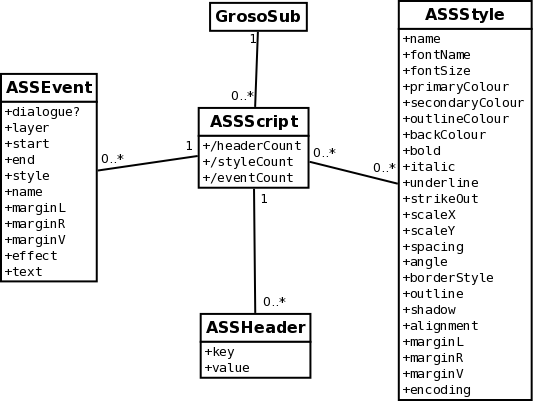
\includegraphics[width=\columnwidth, natwidth=555pt, natheight=402pt]{Pictures/Chapter4/Analisia/DE.png}
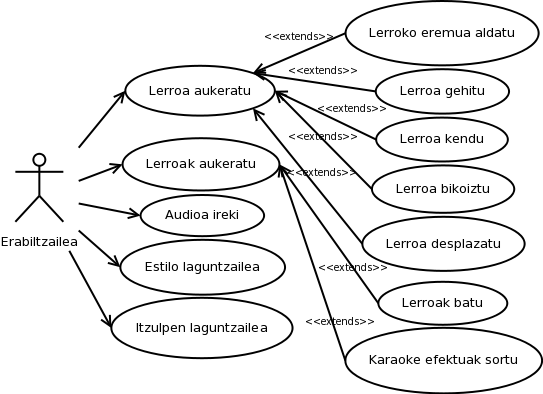
\includegraphics[scale=0.6]{Pictures/Chapter4/Analisia/EKE-Script.png}
\caption{EKE - Script-a irekita egoera}
\label{eke-script}
\end{center}
\end{figure}
\noindent\\
\textbf{ID:} S01.\\
\textbf{Erabilpen kasua:} Lerroa aukeratu.\\
\textbf{Aktoreak:} Erabiltzailea.\\
\textbf{Deskribapena:} Script-ean dagoen lerro bat aukeratzen du ondoren bere gainean zenbait eragiketa egiteko.\\
\textbf{Aurrebaldintzak:}  Script-a kargatuta dago eta gutxienez lerro bat dauka.\\
\textbf{Postbaldintzak:} Lerroa aukeratuta geratzen da.\\
\textbf{Gertaera fluxu normala:}
\begin{enumerate}
	\item \textit{Erabiltzailea:} Script-ean dagoen lerro bat aukeratuko du.
	\item \textit{Sistema:} Erabiltzaileak aukeratutako lerroa markatuko du interfazean.
	\item \textit{Sistema:} Aukeratutako lerroaren datuak kargatuko ditu interfazean (eremuak eta denborak uhin forman audioa kargatuta badago).
\end{enumerate}
\line(1,0){390}\\
\noindent\\
\textbf{ID:} S02.\\
\textbf{Erabilpen kasua:} Lerroko eremua aldatu.\\
\textbf{Aktoreak:} Erabiltzailea.\\
\textbf{Deskribapena:} Aukeratutako lerroko eremu baten edukia aldatzen du.\\
\textbf{Aurrebaldintzak:} Lerro bat aukeratuta dago.\\
\textbf{Postbaldintzak:} Aldatutako eremua lerroan gordeta geratuko da.\\
\textbf{Gertaera fluxu normala:}
\begin{enumerate}
	\item \textit{Sistema:} Aukeratutak lerroaren eremu guztiak eta hauen balioak erakutsiko ditu.
	\item \textit{Erabiltzailea:} Eremu bat aukeratuko du eta honen balioa aldatuko du.
	\item \textit{Erabiltzailea:} Beste eremu bat aldatzeko (2. urratsera) edo aldaketak gordetzeko agindua emango du.
	\item \textit{Sistema:} Lerroan egindako aldaketak gordeko dira.
\end{enumerate}
\line(1,0){390}\\
\noindent\\
\textbf{ID:} S03.\\
\textbf{Erabilpen kasua:} Lerroa gehitu.\\
\textbf{Aktoreak:} Erabiltzailea.\\
\textbf{Deskribapena:} Lerro berri bat gehituko du script-ean.\\
\textbf{Aurrebaldintzak:} Lerro bat aukeratuta dago.\\
\textbf{Postbaldintzak:} Lerro berria script-ean gehituko da.\\
\textbf{Gertaera fluxu normala:}
\begin{enumerate}
	\item \textit{Erabiltzailea:} Aukeratutako lerroaren aurrean edo atzean sartzeko aukeratuko du.
	\item \textit{Sistema:} Erabiltzaileak aukeratutako lekuan txertatuko du lerro berria defektuzko informazioarekin.
\end{enumerate}
\textbf{Gertaera fluxu alternatiboa:}
\begin{itemize}
	\item 0. urratsa: ez badago lerrorik aukeratuta script-ean:
		\begin{enumerate}
		\item \textit{Sistema:} Lerro berri bat gehituko du script-aren amaieran.
		\end{enumerate}
\end{itemize}
\line(1,0){390}\\
\noindent\\
\textbf{ID:} S04.\\
\textbf{Erabilpen kasua:} Lerroa kendu.\\
\textbf{Aktoreak:} Erabiltzailea.\\
\textbf{Deskribapena:} Aukeratutako lerroa script-etik ezabatzen du.\\
\textbf{Aurrebaldintzak:} Lerro bat aukeratuta dago.\\
\textbf{Postbaldintzak:} Lerroa script-etik ezabatuko da.\\
\textbf{Gertaera fluxu normala:}
\begin{enumerate}
	\item \textit{Sistema:} Erabiltzaileak aukeratutako lerroa ezabatuko du script-etik
\end{enumerate}
\line(1,0){390}\\
\noindent\\
\textbf{ID:} S05.\\
\textbf{Erabilpen kasua:} Lerroa bikoiztu.\\
\textbf{Aktoreak:} Erabitzailea.\\
\textbf{Deskribapena:} Aukeratutako lerroaren kopia bat egingo du aukeratutako lerroaren azpian.\\
\textbf{Aurrebaldintzak:} Lerro bat aukeratuta dago.\\
\textbf{Postbaldintzak:} Aukeratutako lerroa bikoiztuta geratuko da.\\
\textbf{Gertaera fluxu normala:}
\begin{enumerate}
	\item \textit{Sistema:} Lerro berri bat sortuko du aukeratutakoaren azpian eta bertan aukeratutako lerroaren datuak sartuko ditu.
\end{enumerate}
\line(1,0){390}\\
\noindent\\
\textbf{ID:} S06.\\
\textbf{Erabilpen kasua:} Lerroak desplazatu.\\
\textbf{Aktoreak:} Erabiltzailea.\\
\textbf{Deskribapena:} Aukeratutako lerroen denborak desplazatzen ditu.\\
\textbf{Aurrebaldintzak:} Gutxienez lerro bat aukeratuta dago.\\
\textbf{Postbaldintzak:} Aukeratutako lerroen denborak desplazatuta geratzen dira.\\
\textbf{Gertaera fluxu normala:}
\begin{enumerate}
	\item \textit{Erabiltzailea:} Desplazatu nahi dituen denborak (hasiera denbora, bukaera denbora edo biak) eta zenbat desplazatu nahi dituen aukeratuko du.
	\item \textit{Sistema:} Aukeratutako lerroen denborak aldatuko ditu erabiltzaileak emandako datuekin.
\end{enumerate}
\line(1,0){390}\\
\noindent\\
\textbf{ID:} S07.\\
\textbf{Erabilpen kasua:} Lerroak aukeratu.\\
\textbf{Aktoreak:} Erabiltzailea.\\
\textbf{Deskribapena:} Script-ean dauden 2 lerro gutxienez aukeratzen ditu ondoren hauen gainean eragiketa bat egiteko.\\
\textbf{Aurrebaldintzak:} Script-a kargatuta dago eta gutxienez 2 lerro ditu.\\
\textbf{Postbaldintzak:} Aukeratutako lerroak markatuta geratuko dira.\\
\textbf{Gertaera fluxu normala:}
\begin{enumerate}
	\item \textit{Erabiltzailea:} Script-ean dauden zenbait lerro aukeratuko ditu.
	\item \textit{Sistema:} Erabiltzaileak aukeratutako lerroak markatuko ditu interfazean.
\end{enumerate}
\line(1,0){390}\\
\noindent\\
\textbf{ID:} S08.\\
\textbf{Erabilpen kasua:} Lerroak batu.\\
\textbf{Aktoreak:} Erabiltzailea.\\
\textbf{Deskribapena:} Aukeratuta dauden lerroak kateatzen ditu.\\
\textbf{Aurrebaldintzak:} 2 lerro gutxienez aukeratuta daude.\\
\textbf{Postbaldintzak:} Aukeratako lerroak kateatuta dituen lerro berri bat sortzen da.\\
\textbf{Gertaera fluxu normala:}
\begin{enumerate}
	\item \textit{Sistema:} Lerro berri bat sortzen du.
	\item \textit{Sistema:} Aukeratutako lerroen edukia (testua) kateatzen du eta denborak egokitzen ditu (hasiera denboren minimoa eta bukaera denboren maximoa).
	\item \textit{Sistema:} Aukeratutako lerroak ezabatzen ditu.
\end{enumerate}
\line(1,0){390}\\
\noindent\\
\textbf{ID:} S09.\\
\textbf{Erabilpen kasua:} Karaoke efektuak sortu.\\
\textbf{Aktoreak:} Erabiltzailea.\\
\textbf{Deskribapena:} Aukeratutako karaoke lerroetan efektuak sortzen ditu.\\
\textbf{Aurrebaldintzak:} Gutxienez lerro bat aukeratuta dago eta karaoke lerroa da.\\
\textbf{Postbaldintzak:} Lerroa eguneratuko da efektuekin.\\
\textbf{Gertaera fluxu normala:}
\begin{enumerate}
	\item \textit{Erabiltzailea:} Ezarri nahi dituen efektuak aukeratuko ditu.
	\item \textit{Sistema:} Efektuak kalkulatuko ditu eta lerroetan gordeko ditu.
\end{enumerate}
\line(1,0){390}\\
\noindent\\
\textbf{ID:} S10.\\
\textbf{Erabilpen kasua:} Audioa ireki.\\
\textbf{Aktoreak:} Erabiltzailea.\\
\textbf{Deskribapena:} Audio fitxategi bat irekitzen du.\\
\textbf{Aurrebaldintzak:} Script-a kargatuta dago.\\
\textbf{Postbaldintzak:} Audioa irekita geratzen da eta bere uhin forma marrazten du.\\
\textbf{Gertaera fluxu normala:}
\begin{enumerate}
	\item \textit{Erabiltzailea:} Fitxategi sisteman dagoen audio fitxategia aukeratzen du.
	\item \textit{Sistema:} Erabiltzaileak aukeratutako fitxategia kargatzen du eta uhin forma marrazten du.
	\item \textit{Sistema:} Audioaren kontrolak aktibatzen ditu (\underline{inclues 15}).
\end{enumerate}
\textbf{Gertaera fluxu alternatiboa:}
\begin{itemize}
	\item 2. urratsa: audio fitxategia ezin da ireki:
		\begin{enumerate}
		\item \textit{Sistema:} Erabiltzaileari errorearen berri emango dio.
		\item \textit{Erabiltzailea:} Audio fitxategi berria aukeratu dezake edo irten daiteke.
		\end{enumerate}
\end{itemize}
\line(1,0){390}\\
\noindent\\
\textbf{ID:} S11.\\
\textbf{Erabilpen kasua:} Estilo laguntzailea.\\
\textbf{Aktoreak:} Erabiltzailea.\\
\textbf{Deskribapena:} Estilo laguntzailea kargatuko du.\\
\textbf{Aurrebaldintzak:} Script-a kargatuta dago.\\
\textbf{Postbaldintzak:} Estilo laguntzailea kargatuko du.\\
\textbf{Gertaera fluxu normala:}
\begin{enumerate}
	\item
\end{enumerate}
\textbf{Gertaera fluxu alternatiboa:}
\begin{itemize}
	\item 
		\begin{enumerate}
		\item
		\end{enumerate}
\end{itemize}
\line(1,0){390}\\
\noindent\\
\textbf{ID:} S12.\\
\textbf{Erabilpen kasua:} Itzulpen laguntzailea.\\
\textbf{Aktoreak:} Erabiltzailea.\\
\textbf{Deskribapena:} Itzulpen laguntzailea kargatuko du.\\
\textbf{Aurrebaldintzak:} Script-a kargatuta dago.\\
\textbf{Postbaldintzak:} Itzulpen laguntzailea kargatuko du.\\
\textbf{Gertaera fluxu normala:}
\begin{enumerate}
	\item
\end{enumerate}
\textbf{Gertaera fluxu alternatiboa:}
\begin{itemize}
	\item 
		\begin{enumerate}
		\item
		\end{enumerate}
\end{itemize}
\newpage


\subsubsection{\textit{Audioa irekita} egoerakoak}
\begin{figure}[htp]
\begin{center}
%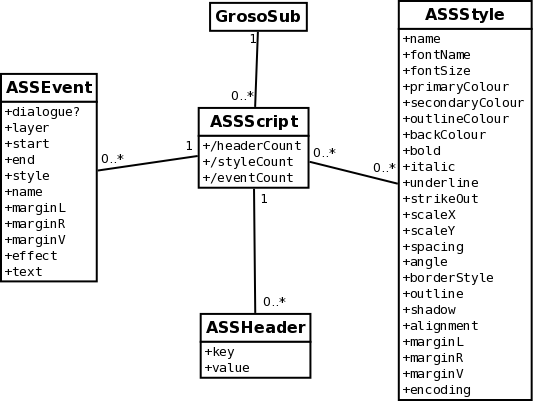
\includegraphics[width=\columnwidth, natwidth=555pt, natheight=402pt]{Pictures/Chapter4/Analisia/DE.png}
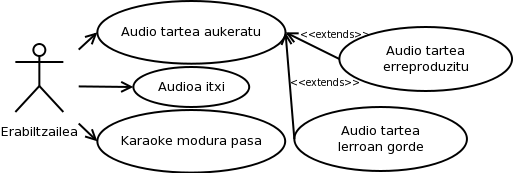
\includegraphics[scale=0.6]{Pictures/Chapter4/Analisia/EKE-Audioa.png}
\caption{EKE - Audioa irekita egoera}
\label{eke-audioa}
\end{center}
\end{figure}
\noindent\\
\textbf{ID:} A01.\\
\textbf{Erabilpen kasua:} Audio tartea aukeratu.\\
\textbf{Aktoreak:} Erabiltzailea.\\
\textbf{Deskribapena:} Kargatutako audioaren tarte bat aukeratzen du beraren gainean zenbait eragiteka egiteko.\\
\textbf{Aurrebaldintzak:} \textit{Audioa irekita} moduan dago programa.\\
\textbf{Postbaldintzak:} Hasiera eta bukaera denborak finkatuta geratzen dira.\\
\textbf{Gertaera fluxu normala:}
\begin{enumerate}
	\item \textit{Erabiltzailea:} Uhin formaren gainean hasiera eta bukaera denborak ezartzen ditu.
	\item \textit{Sistema:} Aukeratutako tartea baliozkoa dela begiratu ondoren tartea gordetzen du.
\end{enumerate}
\line(1,0){390}\\
\noindent\\
\textbf{ID:} A02.\\
\textbf{Erabilpen kasua:} Audio tartea erreproduzitu.\\
\textbf{Aktoreak:} Erabiltzailea.\\
\textbf{Deskribapena:} Aukeratutako audio tartea erreproduzitzen du espezifikatutako moduan.\\
\textbf{Aurrebaldintzak:} Audio tartea aukeratuta dago.\\
\textbf{Postbaldintzak:} Audio erreproduzitzen da.\\
\textbf{Gertaera fluxu normala:}
\begin{enumerate}
	\item \textit{Erabiltzailea:} Erreproduzitzeko modua aukeratzen du.
	\item \textit{Sistema:} Erabiltzaileak aukeratutako moduan erreproduzitzen du audio tartea.
\end{enumerate}
\line(1,0){390}\\
\noindent\\
\textbf{ID:} A03.\\
\textbf{Erabilpen kasua:} Audio tartea lerroan gorde.\\
\textbf{Aktoreak:} Erabiltzailea.\\
\textbf{Deskribapena:} Aukeratutako audio artea aukeratutako lerroan gordetzen du.\\
\textbf{Aurrebaldintzak:} Audio tartea eta lerro bat aukeratuta daude.\\
\textbf{Postbaldintzak:} Audio tartea aukeratutako lerroan gordetzen da.\\
\textbf{Gertaera fluxu normala:}
\begin{enumerate}
	\item \textit{Sistema:} Uhin formaren gainean aukeratutako denbora tartea aukeratutako lerroan gordetzen du.
\end{enumerate}
\line(1,0){390}\\
\noindent\\
\textbf{ID:} A04.\\
\textbf{Erabilpen kasua:} Audio itxi.\\
\textbf{Aktoreak:} Erabiltzailea.\\
\textbf{Deskribapena:} Irekita dagoen audio ixten du.\\
\textbf{Aurrebaldintzak:} Audioa kargatuta dago.\\
\textbf{Postbaldintzak:} Audioa itxita geratzen da eta audio moduko kontrolak ezkutatzen dira.\\
\textbf{Gertaera fluxu normala:}
\begin{enumerate}
	\item \textit{Sistema:} Audio ixten du eta kontrolak ezkutatzen ditu.
\end{enumerate}
\line(1,0){390}\\
\noindent\\
\textbf{ID:} A05.\\
\textbf{Erabilpen kasua:} Karaoke modura pasa.\\
\textbf{Aktoreak:} Erabiltzailea.\\
\textbf{Deskribapena:} Karaokeak sinkronizatzeko modura pasatzen da.\\
\textbf{Aurrebaldintzak:} Audioa kargatuta dago.\\
\textbf{Postbaldintzak:} Karaokeak sinkronizatzeko kontrolak aktibatzen dira.\\
\textbf{Gertaera fluxu normala:}
\begin{enumerate}
	\item \textit{Sistema:} Audioaren kontrolak ezkutatzen ditu eta karaokeak sinkronizatzeko kontrolak aktibatzen ditu.
	\item \textit{Sistema:} Lerroan dauden zatiak uhin formaren gainean marrazten ditu.
\end{enumerate}
\newpage


\subsubsection{\textit{Karaoke modua} egoerakoak}
\begin{figure}[htp]
\begin{center}
%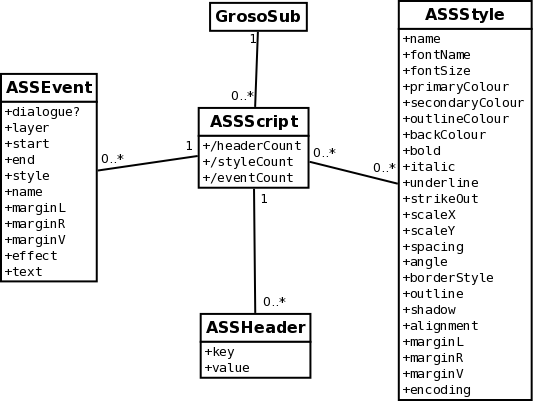
\includegraphics[width=\columnwidth, natwidth=555pt, natheight=402pt]{Pictures/Chapter4/Analisia/DE.png}
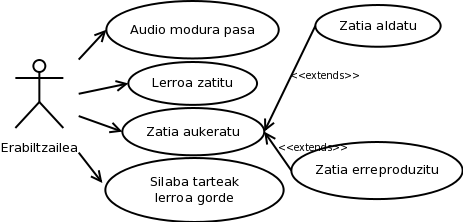
\includegraphics[scale=0.6]{Pictures/Chapter4/Analisia/EKE-Karaoke.png}
\caption{EKE - Karaoke modua egoera}
\label{eke-karaoke}
\end{center}
\end{figure}
\noindent\\
\textbf{ID:} K01.\\
\textbf{Erabilpen kasua:} Audio modura pasa.\\
\textbf{Aktoreak:} Erabiltzailea.\\
\textbf{Deskribapena:} Audio modura pasatzen da, lerroen denborak ezartzeko modua.\\
\textbf{Aurrebaldintzak:} Audioa kargatuta dago.\\
\textbf{Postbaldintzak:} Audio moduko kontrolak aktibatzen ditu.\\
\textbf{Gertaera fluxu normala:}
\begin{enumerate}
	\item \textit{Sistema:} Audio moduko kontrolak erakusten ditu.
\end{enumerate}
\line(1,0){390}\\
\noindent\\
\textbf{ID:} K02.\\
\textbf{Erabilpen kasua:} Lerroa zatitu.\\
\textbf{Aktoreak:} Erabiltzailea.\\
\textbf{Deskribapena:} Aukeratutako lerroa silabaka zatitzen du.\\
\textbf{Aurrebaldintzak:} Karaoke moduan dago programa eta lerro bat aukeratuta dago.\\
\textbf{Postbaldintzak:} Lerroaren silabak zatituta geratzen dira.\\
\textbf{Gertaera fluxu normala:}
\begin{enumerate}
	\item \textit{Erabiltzailea:} Lerroaren silabak zeintzuk diren adierazioko du.
	\item \textit{Sistema:} Lerroa erabiltzaileak emandako silabatan zatituko du.
\end{enumerate}
\line(1,0){390}\\
\noindent\\
\textbf{ID:} K03.\\
\textbf{Erabilpen kasua:} Zatia aukeratu.\\
\textbf{Aktoreak:} Erabiltzailea.\\
\textbf{Deskribapena:} Lerroaren zati bat aukeratzen du.\\
\textbf{Aurrebaldintzak:} Karaoke moduan dago programa eta lerro bat aukeratuta dago.\\
\textbf{Postbaldintzak:} Zatia aukeratuta geratzen da.\\
\textbf{Gertaera fluxu normala:}
\begin{enumerate}
	\item \textit{Erabiltzailea:} Lerroko zati bat aukeratzen du.
	\item \textit{Sistema:} Erabiltzaileak aukeratutako zatia markatzen du interfazean.
\end{enumerate}
\line(1,0){390}\\
\noindent\\
\textbf{ID:} K04.\\
\textbf{Erabilpen kasua:} Zatia aldatu.\\
\textbf{Aktoreak:} Erabiltzailea.\\
\textbf{Deskribapena:} Aukeratutako zatiaren hasiera eta bukaera denborak aldatzen ditu.\\
\textbf{Aurrebaldintzak:} Zati bat aukeratuta dago.\\
\textbf{Postbaldintzak:} Zatiaren eta ondokoen denborak aldatuta geratzen dira.\\
\textbf{Gertaera fluxu normala:}
\begin{enumerate}
	\item \textit{Erabiltzailea:} Uhin formaren gainean zatiaren hasiera eta bukaera denborak ezartzen ditu.
	\item \textit{Sistema:} Zatiaren eta ondokoen denborak eguneratzen dira.
\end{enumerate}
\line(1,0){390}\\
\noindent\\
\textbf{ID:} K05.\\
\textbf{Erabilpen kasua:} Zatia erreproduzitu.\\
\textbf{Aktoreak:} Erabiltzailea.\\
\textbf{Deskribapena:} Aukeratutako zatia erroproduzitzen du.\\
\textbf{Aurrebaldintzak:} Zati bat aukeratuta dago.\\
\textbf{Postbaldintzak:} Aukeratutako zatia erreproduzitzen du.\\
\textbf{Gertaera fluxu normala:}
\begin{enumerate}
	\item \textit{Sistema:} Aukeratutako dagoen zatia erreproduzitzen du.
\end{enumerate}
\line(1,0){390}\\
\noindent\\
\textbf{ID:} K06.\\
\textbf{Erabilpen kasua:} Silaba tarteak lerroan gorde.\\
\textbf{Aktoreak:} Erabiltzailea.\\
\textbf{Deskribapena:} Silaba tarteak lerroan gordetzen ditu.\\
\textbf{Aurrebaldintzak:} Programa karaoke moduan dago eta lerro bat aukeratuta dago.\\
\textbf{Postbaldintzak:} Silaba tarteak lerroan gordeta geratzen dira.\\
\textbf{Gertaera fluxu normala:}
\begin{enumerate}
	\item \textit{Sistema:} Erabiltzaileak ezarritako silaba tarteak lerroan gordetzen ditu.
\end{enumerate}

\section{Diseinua}
\subsection{Dokumentuetan oinarritutako aplikazioak}
Gure aplikazioak oso komunak diren funtzionalitate batzuk izan behar ditu: fitxategiak ireki, berriak sortu, itxi, etab. Aplikazio hauek dokumentuetan oinarritutakoak dira, eta oso komunak direnez, Cocoa API-ak hauek garatzeko erreztasun asko ematen ditu. \textbf{MVC}\footnote{Model View Controller} patroia jarraituko da diseinua egiterako orduan, nahiz eta klase batzuk mota bat baino gehiagokoak izango diren aurrerago ikusiko dugunez.
\subsubsection{Dokumentu arkitektura}
Horrelako aplikazioak gauzatzeko hiru klase eskaintzen ditu Cocoa-k. Lehenik eta behin \texttt{NSDocument} klasea daukagu. Honen azpiklase bat sortuko dugu dokumentuaren (ASS fitxategia gure kasuan) egitura gordetzeko. Nahiz eta zenbait dokumentu formatu onartuko dituen programak (ASS, SRT eta TXT), ASS-rekin lan egingo du barrutik, beraz azpiklase bakarra sortuko dugu. Klase hau \textit{Model} eta \textit{Controller} motakoa izango da.

Ondoren \texttt{NSWindowController} klasea daukagu. Sortuko dugun aplikazioak lehio bakarra edukiko badu, honen azpiklasea egitea ez da beharrezkoa izango. Gure kasuan lehio bat baino gehiago edukiko dugu dokumentu bakar batentzako, beraz lehio mota bakoitzeko azpiklase bat sortuko dugu. Klaseak interfazearen ekintzak jasoko ditu eta \textit{Model} klasea eguneratuko du. Gainera, azpiklase bakoitza \textbf{NIB} fitxategi konkretu batera lotuta egongo da, non interfazea gordeko den (modu grafikoan editatzen dira fitxategi hauek interfaze grafikoa osatzeko). Hau \textit{Controller} motako klasea da.

Azkenik \texttt{NSDocumentController} klasearekin aurkituko gara, baina honen azpiklaserik ez dugu beharko. Honen eginkizuna dokumentuak maneiatzea da: berriak sortzea, ixtea, etab.

\subsubsection{Ohiko atazak}
Lehen esan bezala, badaude programa hauetan oso ohikoak diren funtzionalitate batzuk, eta dokumentu arkitekturak lana asko errazten digu hauek inplementatzeko. \texttt{NSDocument}-en azpiklasean bi metodo inplementatu beharko dira:
\begin{itemize}
\item \texttt{-dataOfType:error:}:

\texttt{NSData} motako objektu bat (\texttt{NSString} bat kodifikazioa espezifiko batekin, \textbf{UTF8} gure kasuan) itzuli behar du dokumentuaren edukiarekin fitxategi batean gordetzeko. \texttt{typeName} parametroarekin jakingo dugu zein den fitxategiaren formatua.

\item \texttt{-readFromData:ofType:error:}:

\texttt{NSData} motako objektu bat eta fitxategiaren formatua jasotzen du. Bere eginkizuna zera da: edukia irakurtzea eta dokumentuko datu egiturak betetzea.
\end{itemize}

Erabilpen kasu hauen sekuentzia diagramak ez dira egingo: G01 - Fitxategia ireki, G02 - Script berria sortu eta G03 - Fitxategia gorde, Apple-en dokumentazioan\footnote{Apple-en dokumentazioko\cite{ap:dba} 29. orrialdean} aurkitu daitezkeelako, nahiz eta apur bat zahartuta egon (goian aipatutako metodoak ez dira erabiltzen, hauen ordez apur bat zaharragoak baina eginkizun berdina dutenak erabiltzen dira).

Sekuentzia diagramak ikusita, guk oso gutxi programatu beharko dugu (bi funtzio) fitxategiak ireki, itxi eta gordetzeko, kode asko aurreztuz (adibidez ez dugu fitxategia aukeratzeko panela maneiatu beharko edo dokumentuaren instantzia berria sortu beharko).

\subsubsection{Desegin/Berregin}
Aukera hauek inplementatzeko dokumentu arkitekturak ere lana asko erreztuko digu. \texttt{NSDocument}-ek \texttt{NSUndoManager} en instantzia bat dauka. Adibidez, aplikazioan lerro berri bat gehitzen dugunean, \texttt{NSUndoManager}-ean kontrako ekintza erregistratuko dugu, kasu honetan lerroa kentzea. Azken finean bi pila dauzka \texttt{NSUndoManager}-ek, bat desegiteko ekintzekin eta beste bat berregiteko ekintzekin. Desegitea aukeratzen dugunean, berregiteko pilan txertatuko da kontrako ekintza eta alderantziz. Menuko aukerak ere automatikoki kudeatuko dira guk ezer egin gabe.

\subsubsection{Dokumentuaren egoera}
Dokumentuan aldaketaren bat egin badugu, dokumentuaren aldaketa kontagailua inkrementatuko dugu. Kontagailu hau 0 ez bada, dokumentua zikin dagoela esango dugu, hau da, fitxategi sisteman dagoen fitxategia eta aplikazioan kargatuta dagoen dokumentua ez dira berdinak. Programa ixten saiatzen bagara, mezu bat agertuko zaigu zer egin nahi dugun galdetuz (gorde, ez gorde edo ezeztatu).

Aldaketaren bat desegiten badugu, kontagailua murriztuko da, eta fitxategia gordetzen badugu, kontagailuaren balioa 0 izango da berriz ere.

Aurreko kasuetan bezala, esfortzu gutxirekin (kode lerrorik gabe), funtzionalitate hau inplementatuta edukiko dugu.

\subsubsection{Informazio gehiago}
Atal honetan ikusi dugunez, erraztasun asko ematen dizkigu dokumentu arkitekturak, baina askoz gauza gehiago egiteko ere gai da. Informazio gehiago aurkitu daiteke Apple-ek eskaintzen duen dokumentazioan\cite{ap:dba}.

\subsection{Sekuentzia diagramak}

\section{Inplementazioa}

\section{Probak}

\section{Kudeaketa}